\documentclass{pnas-new}
\templatetype{pnasresearcharticle}

%% PNAS_Logo.pdf and class files live in PNAS_guidelines/
\graphicspath{{figures/}}

\usepackage{amsmath}
\usepackage{booktabs}
\usepackage{float}

%% ── Title & authors ──────────────────────────────────────────────────────────
\title{Climate and the molecular evolution of Influenza A surface proteins}

\author[1]{Nina Pust}

\affil[1]{Department of Veterinary and Animal Sciences, University of Copenhagen, Copenhagen, Denmark}

\leadauthor{Pust}

\correspondingauthor{\textsuperscript{1}Correspondence: nina.pust@sund.ku.dk}

\keywords{influenza A | hemagglutinin | molecular evolution | climate | phylogenetic comparative methods}

\dates{Submitted: \today}

\doi{\url{https://doi.org/10.XXXX/pnas.XXXXXXXXXX}}

%% ── Significance statement (≤ 120 words, plain language) ────────────────────
\significancestatement{%
Influenza A is a major cause of seasonal epidemics and occasional pandemics.
Understanding what drives the emergence of novel variants is critical for
pandemic preparedness and vaccine design. We link local environmental
temperature to the rate of molecular evolution in influenza A haemagglutinin
(HA) using a global surveillance dataset spanning 2009--2019. Colder
conditions are associated with accelerated HA evolution in both H1N1 and
H3N2, consistent with climate modulating within-host viral population sizes
or transmission bottlenecks rather than directly steering adaptive change.
These results suggest that geographic and seasonal patterns of HA evolution
are partly climatically determined, with implications for understanding how
global climate change may reshape the distribution of influenza evolutionary
hotspots.}

%% ── Author contributions etc. ────────────────────────────────────────────────
\authorcontributions{N.P.\ designed and performed the analysis and wrote the manuscript.}
\authordeclaration{The authors declare no competing interest.}

% ─────────────────────────────────────────────────────────────────────────────
\begin{document}
\maketitle

% ─────────────────────────────────────────────────────────────────────────────
\begin{abstract}
Influenza A infections display marked seasonal patterns, peaking in winter
months in temperate regions and in rainy seasons in the tropics.
Environmental conditions are thought to influence viral transmission and
host immunity, yet direct evidence linking climate to molecular evolutionary
rates remains limited. Here we use phylogenetic comparative regression
applied to a global dataset of \textbf{[X]} hemagglutinin (HA),
neuraminidase (NA) and polymerase acidic protein (PA) sequences from H1N1
and H3N2, collected between 2009 and 2019, to test whether local temperature,
relative humidity, and population density predict substitution rates.
Temperature shows a significant negative association with HA substitution
rate, affecting synonymous and non-synonymous rates equally and persisting
across antigenic subregions of H1. No equivalent association is detected in
NA or in the PA negative control. Individual amino acid substitutions in
antigenic sites show no enrichment in colder or drier climates, indicating
that temperature accelerates the HA evolutionary clock without biasing the
direction of antigenic change. These findings suggest that cold conditions
enlarge the mutational supply available for immune escape, and that climate
change may consequently alter the geographic distribution of influenza
evolutionary hotspots.
\end{abstract}

% ─────────────────────────────────────────────────────────────────────────────
\section*{Introduction}

Influenza A infections display marked seasonal patterns, peaking in winter
months in temperate regions and in rainy seasons in the tropics
\citep{petrova_evolution_2018}, also causing devastating epidemics and most
of the major pandemics in the last century
\citep{hsieh_influenza_2006, trovao_when_2020}. Local climates are likely
to be involved in variant emergence by influencing mode of transmission,
host immunity and respiratory tract conditions \citep{kudo_low_2019}.
Climatic conditions that allow greater droplet stability can relax the
population bottleneck at transmission \citep{frise_contact_2016}, reducing
the loss of novel variants during host-to-host spread. Experimental work has
shown that colder and drier conditions increase transmission efficiency due
to enhanced virus survival in airborne droplets
\citep{lowen_influenza_2007, shaman_absolute_2009}. Meanwhile, hot and
humid conditions might also promote viral survival by reducing desiccation
\citep{minhaz_ud-dean_structural_2010}, such that the role of climate on
variant emergence is likely complex \citep{deyle_global_2016} and remains
poorly understood. Modern global-scale surveillance data frequently includes
genetic sequences for the core hemagglutinin (HA) and neuraminidase (NA)
viral surface protein genes, which provide fundamental information about
strain emergence in addition to date and location of collection, even in
the absence of additional patient information \citep{volz_viral_2013}.

The influenza viral surface proteins HA and NA are fast-evolving and
directly involved in transmission and infection efficiency
\citep{nelson_evolution_2007}. HA binds to sialic acid on host glycoproteins
or glycolipids, facilitating viral entry into the host cell. Meanwhile, NA
cleaves sialic acids on host and virion glycoproteins, enabling the release
of virions from the host cells \citep{matsuoka_comprehensive_2013}. The
function of both of these surface proteins can be acutely affected by
extracellular environmental conditions, in particular pH
\citep{klenow_influenza_2023, tosheva_hemagglutinin_2023}, pointing to
strong selection pressures prior to cell access. Variants that require a
lower pH for the activation of HA are thought to have a selective advantage
in transmission, as they are less susceptible to inactivation in mildly
acidic extracellular environments
\citep{russier_molecular_2016, singanayagam_influenza_2019, tosheva_hemagglutinin_2023}.
Meanwhile, colder and drier conditions reduce mucus transport velocity
\citep{kelly_rapid_2021, kilgour_mucociliary_2004} and likely pH in airways
\citep{kullmann_environmental_2008}.

Dry air additionally impairs innate antiviral defence and tissue repair,
making regions with driest climates likely to worsen susceptibility to
severe disease \citep{kudo_low_2019}. Environmental temperature and humidity
might therefore impact viral evolution via changed infection times, viral
loads, and selection pressures mediated by factors like airway mucus
composition. Alternatively, outdoor environmental climate might not be a
relevant predictor of viral novelty — this might occur if evolution is
dominated by the intracellular environment \citep{partlow_influenza_2025} or
by demographic patterns of transmission driven by social habits and networks
\citep{cauchemez_role_2011, endo_within_2021}.

In RNA viruses like influenza A, mutational genetic change, known as
antigenic drift, is shaped by multiple factors including mutation rates,
replication dynamics, and host immune pressures
\citep{nelson_evolution_2007, wille_ecology_2020}. Antigenic drift,
influenced by host immunity and vaccination, is a potent driver of novel
strain emergence in influenza \citep{bedford_integrating_2014}, along with
reassortment events between co-occurring lineages (i.e., antigenic shift)
\citep{nelson_evolution_2007}. Environmental conditions can influence
evolutionary rates either directly via physical conditions for virion
survival, or indirectly by altering social dynamics and people movement.
Global climate change might therefore alter the prevalence and geographic
distribution of evolutionary hotspots, likely causing more recurrent or
ongoing outbreaks compared to the seasonal peaks currently observed in
temperate regions \citep{baker_implications_2021}.

In this study, we use a global data set of influenza A to test for the
links between local climate, population density, and rates of molecular
evolution of surface antigens in the two most common seasonal strains:
H1N1 and H3N2. Additionally, we use the polymerase acidic protein gene
(PA), an internal, slow-evolving gene, as a negative control. Using a
dataset with over \textbf{[X]} surveillance samples of each gene, sampled
globally across two strains, we inferred terminal branch rates and
non-synonymous and synonymous substitution rates per sample. Comparative
analysis was then performed on these data to test for fundamental climatic
or demographic predictors of evolutionary rates. By characterising how
climate influences viral evolutionary dynamics, we propose hypotheses for
the formation of influenza A evolutionary hotspots and seasonal peaks under
global climatic change.

% ─────────────────────────────────────────────────────────────────────────────
\section*{Results}

To assess whether local climate conditions shape influenza A evolution, we
applied phylogenetic comparative regression to substitution rates estimated
across H1N1 and H3N2 sequences spanning 2009--2019 across 168 countries
(Fig.~\ref{fig:main}A). Surface proteins HA and NA were tested due to their
fast-evolving nature and key role in immune escape, while PA served as a
negative control. To account for the confounding seasonal burden of
influenza A infections in winter months, sampling density was included as a
covariate. The results reveal that HA sequences collected at higher
temperature show a decreased substitution rate (Fig.~\ref{fig:main}C). This
effect was not observed in NA or PA.

\begin{figure*}[bt!]
  \centering
  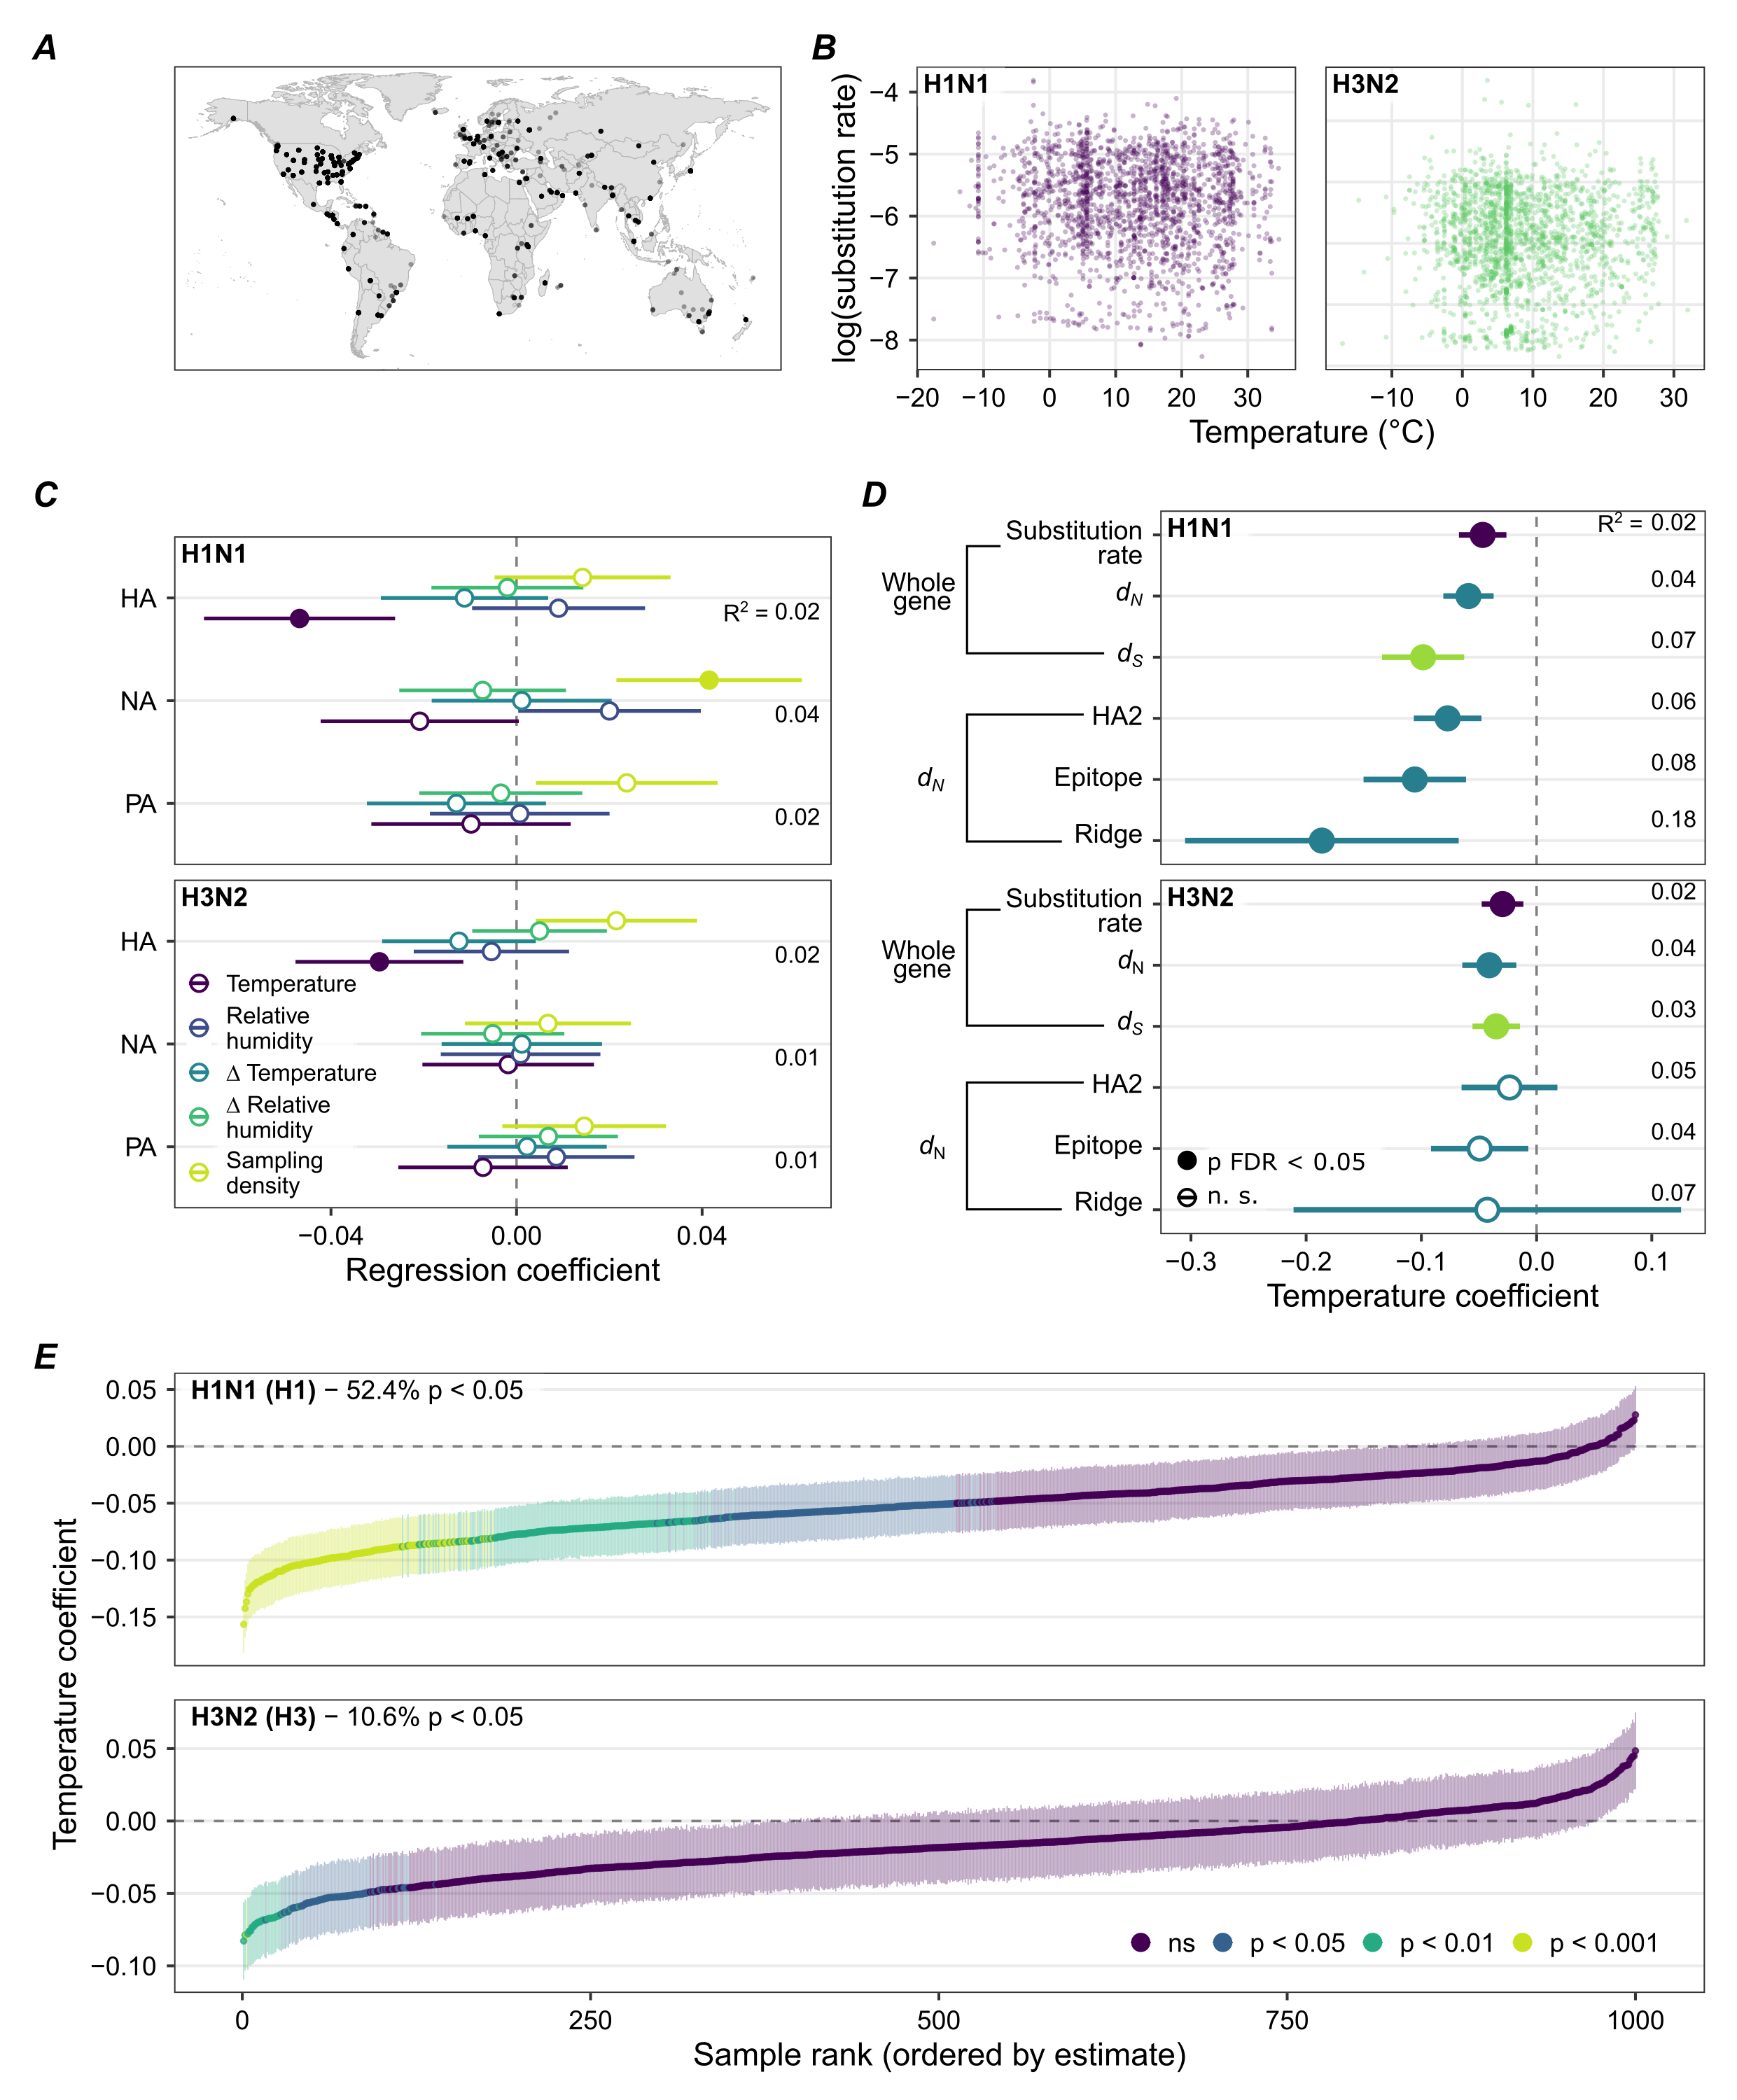
\includegraphics[width=\textwidth]{fig1_mod.png}
  \caption{\textbf{(A)} Global distribution of H1N1 and H3N2 sequences used
    in the analysis. \textbf{(B)} Overall substitution rate and temperature
    of each H1N1 and H3N2 sample. \textbf{(C)} Phylogenetic regression
    coefficients for the association between each climate predictor and the
    overall substitution rate with 95\% confidence intervals. Filled symbols
    indicate associations significant after Benjamini--Hochberg FDR
    correction ($p_{\text{FDR}} < 0.05$). \textbf{(D)} Regression
    coefficients for temperature, split by antigenic ridge, broader epitope
    region, and stalk region (HA2). Filled symbols indicate FDR-significant
    associations. \textbf{(E)} Block jackknife sensitivity analysis:
    regression coefficients for temperature estimated after subsampling 1000
    sequences from the dataset 1000 times, confirming that results are not
    driven by any single sequence or set of sequences.}
  \label{fig:main}
\end{figure*}

To further investigate the impact of temperature on HA substitution rate,
the rate of synonymous ($d_{\text{S}}$) and non-synonymous ($d_{\text{N}}$)
change was analysed across the whole gene, the stalk region (HA2), the
epitope regions, and the antigenic ridge (see \textcolor{red}{Supp.\ Fig.\ gene map}).
No notable difference was observed between the $d_{\text{N}}$, $d_{\text{S}}$
and overall substitution rates across both analysed subtypes
(Fig.~\ref{fig:main}D), implying that temperature plays a role in mutational
rate but does not influence selection. Analyses on the stalk region (HA2),
epitope regions, and the antigenic ridge showed that the temperature signal
persists across gene regions of H1, while H3 does not reach significance in
these analyses. This could be due to the reduced statistical power of
restricting to sequences that have undergone a non-synonymous change in each
respective gene region, along with the fact that the overall regression
analysis was less significant in H3N2 than in H1N1
($p_{\text{FDR(H1N1)}} = \text{value}$, $p_{\text{FDR(H3N2)}} = \text{value}$).

A similar trend is apparent in the block jackknife sensitivity analysis,
showing that temperature has a significant negative effect on H1 in 52\% of
subsamples but only in 10\% in H3 (Fig.~\ref{fig:main}E). Furthermore,
this analysis revealed that the temperature signal was not driven by any
particular sequence or set of sequences, but rather distributed evenly
across the dataset (\textcolor{red}{Supp.\ Fig.\ per-sequence jackknives}).

An in-depth analysis of non-synonymous mutations on the antigenic ridge and
epitope regions of H1 and H3 revealed that several amino acid substitutions
occur independently multiple times across taxa (Fig.~\ref{fig:mutations},
top row). However, a Wilcoxon rank-sum test reveals that no association
between each substitution and each climate variable reaches statistical
significance (Fig.~\ref{fig:mutations}, bottom row).

\begin{figure*}[bt!]
  \centering
  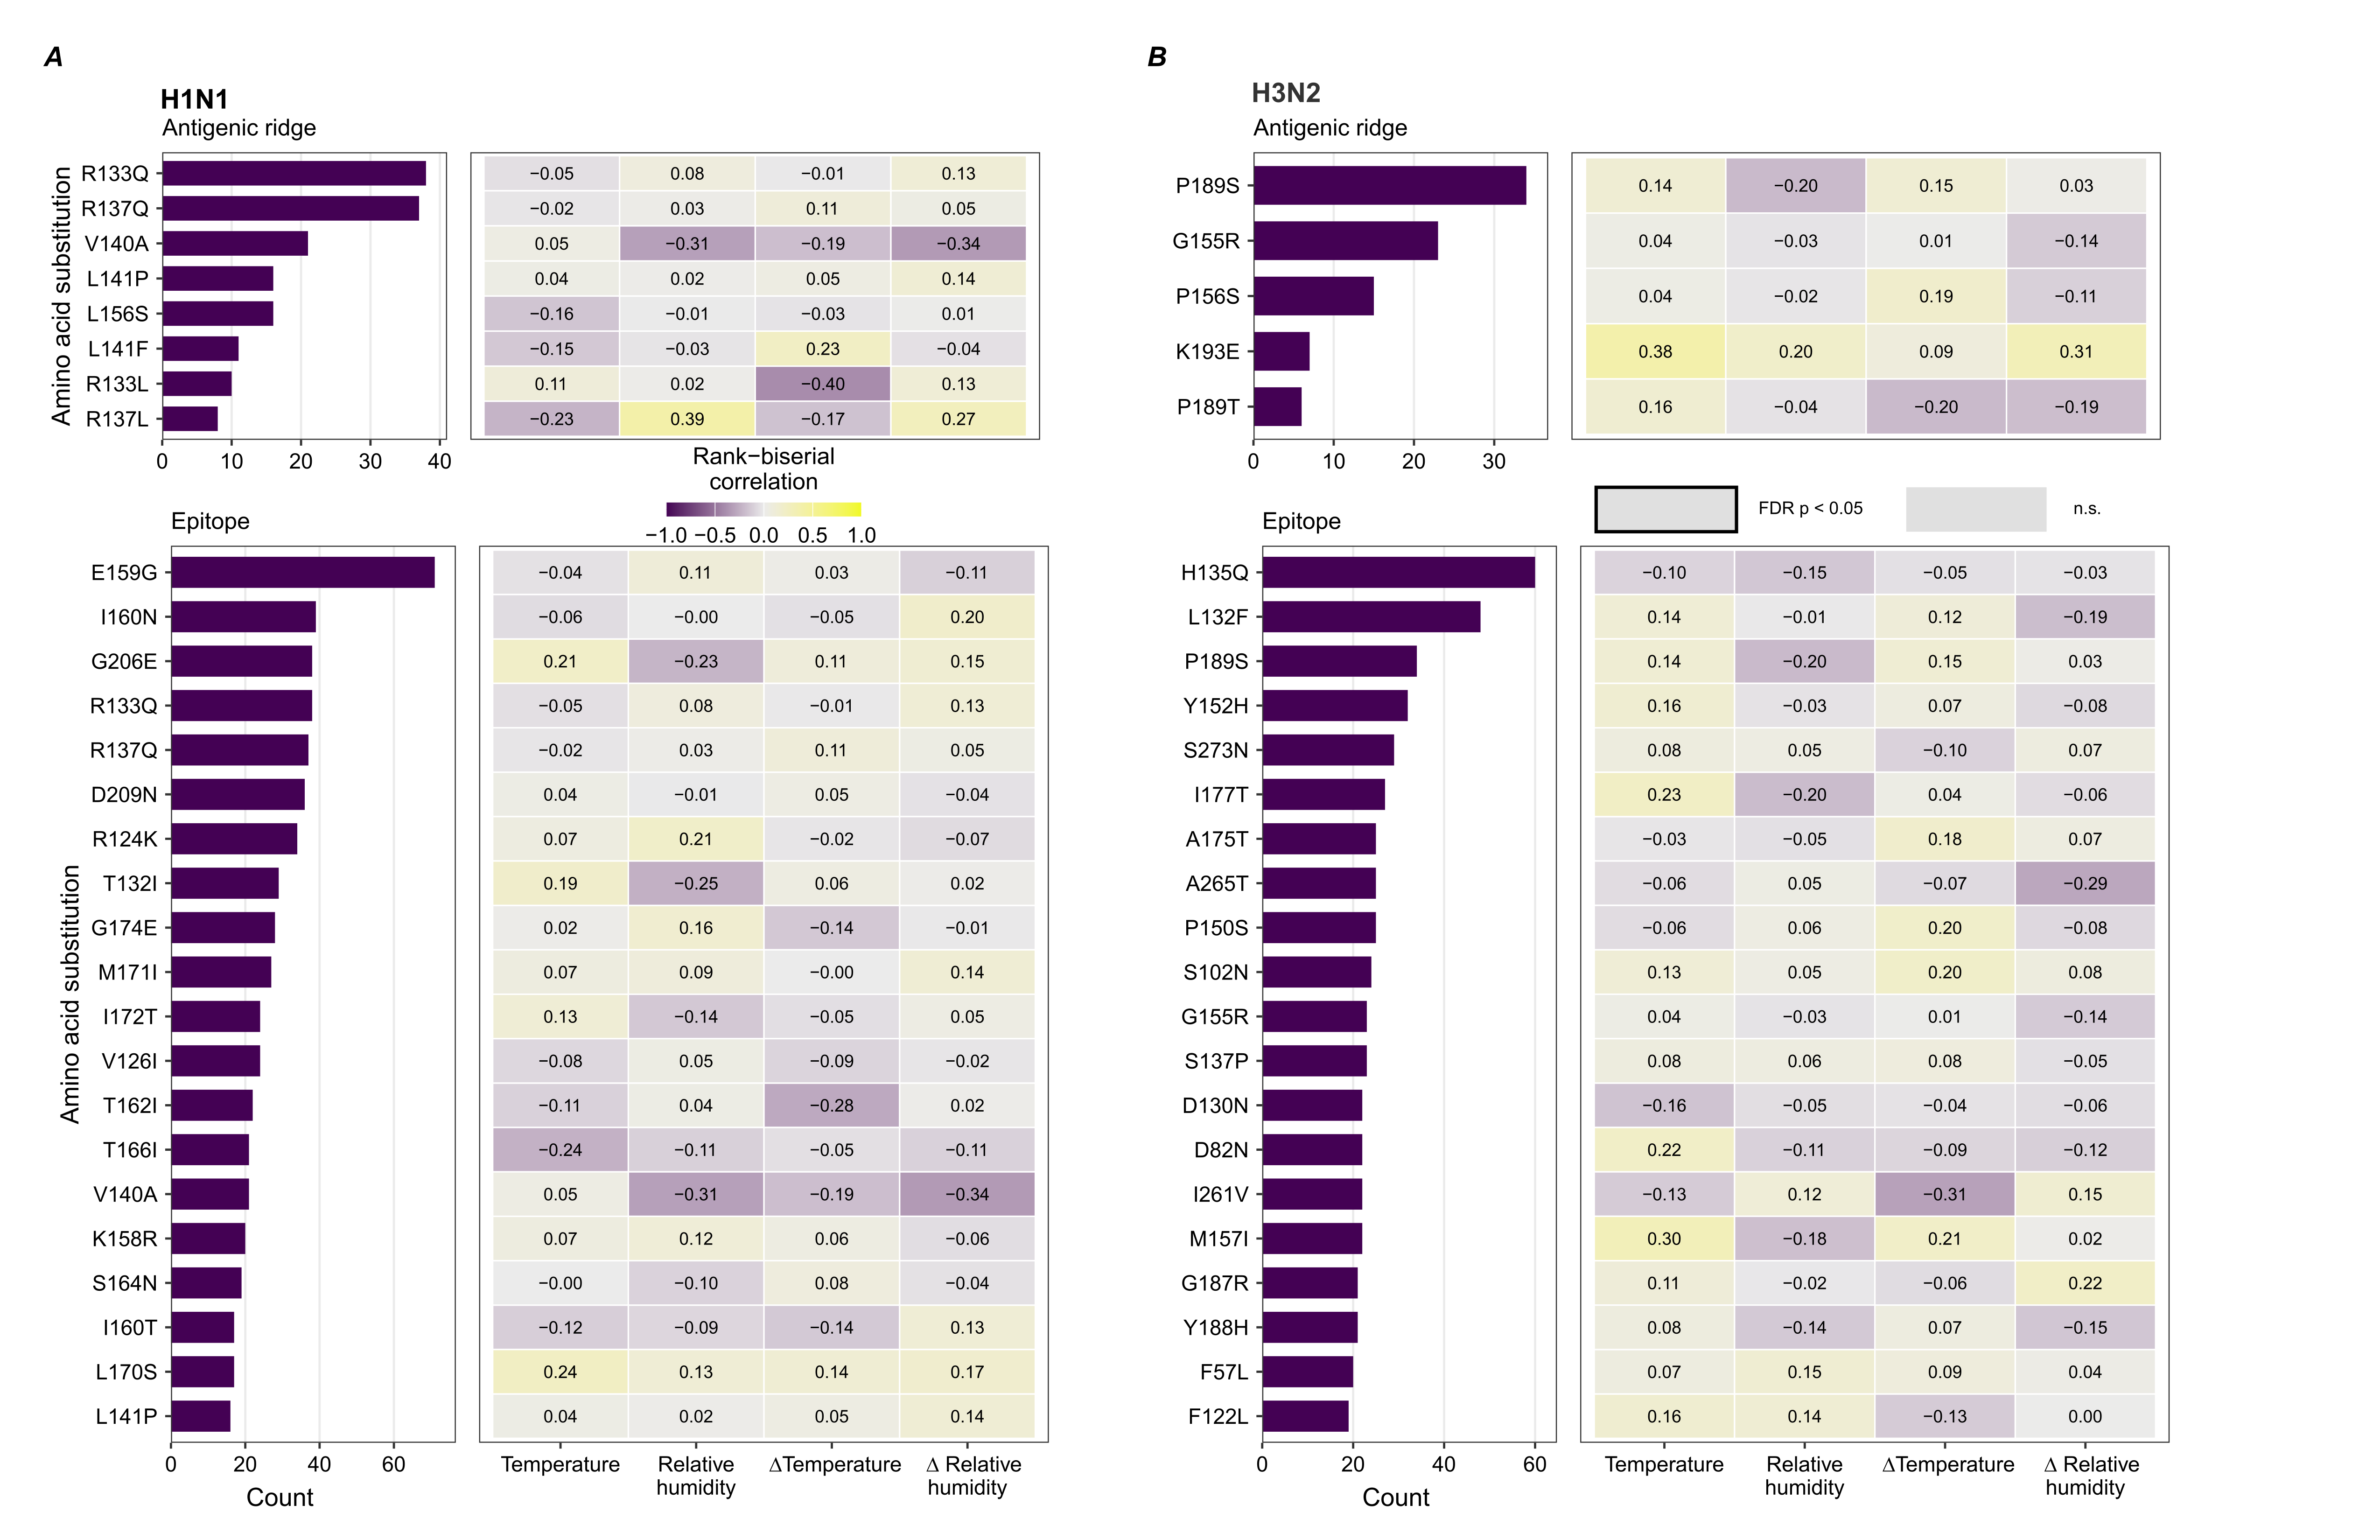
\includegraphics[width=\textwidth]{fig2_mutations_mod.png}
  \caption{\textbf{Recurrent amino acid substitutions in the antigenic ridge
    and epitope regions do not show climate-specific enrichment.}
    Bar plots (left of each panel pair) show the number of independent
    evolutionary occurrences of each amino acid substitution (occurrences
    $> 5$) in the haemagglutinin antigenic ridge (top row) and the broader
    epitope region (bottom row; 20 most frequent substitutions shown) for
    H1N1 (\textbf{A}) and H3N2 (\textbf{B}). Heatmaps (right of each panel
    pair) display the rank-biserial correlation between each climate variable
    (temperature, relative humidity, and their seasonal deltas) and the
    presence or absence of each substitution, estimated by a Wilcoxon
    rank-sum test. No substitution reaches statistical significance after
    Benjamini--Hochberg false discovery rate correction (FDR $< 0.05$; black
    tile border), indicating that climate does not selectively drive any
    specific amino acid change in the antigenic surface of HA.}
  \label{fig:mutations}
\end{figure*}

% ─────────────────────────────────────────────────────────────────────────────
\section*{Discussion}

\begin{itemize}

    \item \textbf{Restate the core finding and its novelty.}
    Open by briefly summarising what was found: a significant negative
    association between local temperature and HA substitution rate in both
    H1N1 and H3N2, robust to subsampling, not driven by any single sequence
    or outbreak cluster. Situate this in the literature — prior work has
    linked climate to influenza \emph{transmission}, but direct evidence
    linking ambient conditions to evolutionary rate in a global dataset is
    limited. This is the contribution.

    \item \textbf{Interpret the direction: cold $\rightarrow$ faster
    evolution.} Discuss that the direction is consistent with the
    well-established winter-season dominance in temperate regions. Cold
    conditions are associated with drier indoor air, longer outdoor aerosol
    persistence, reduced mucociliary clearance, and potentially lower airway
    pH — all of which may extend the transmission bottleneck window and
    expose a larger within-host viral population to selection. Faster
    replication cycles or larger effective population sizes at transmission
    could manifest as an elevated substitution rate at the population level
    even without a change in per-replication error rate.

    \item \textbf{Why both $d_\text{N}$ and $d_\text{S}$? Mutational rate,
    not altered selection.} The lack of a differential effect on $\omega$
    ($d_\text{N}/d_\text{S}$) and the fact that the signal persists in
    synonymous as well as non-synonymous rates suggests that temperature is
    modulating the overall rate of molecular change rather than the
    \emph{type} of change. A plausible interpretation is that colder, drier
    conditions lead to larger within-host population sizes or more
    replication rounds per transmission chain, generating more raw
    mutations — both synonymous and non-synonymous — without specifically
    enriching for adaptive change. This interpretation is also consistent
    with the mutation-frequency analysis showing no specific amino acid
    substitution enriched in colder climates.

    \item \textbf{Why HA and not NA or PA?} HA is the primary target of
    humoral immunity and is under strong immune-driven positive selection,
    meaning it has the most headroom for variation. Possible explanations:
    (1) HA faces direct extracellular selection pressure (pH, mucus,
    antibody) that amplifies any climate-induced change in mutational supply;
    (2) NA evolves under different immune and functional constraints and may
    be subject to epistatic coupling with HA that buffers its rate; (3) the
    PA negative-control result confirms the pipeline is not generating
    spurious signals, and the NA null result is biologically informative
    rather than a power failure (NA sample sizes are comparable). Worth
    briefly considering whether the HA--climate link is HA-specific or just
    a consequence of HA evolving fastest overall, making small
    climate-linked differences easier to detect.

    \item \textbf{Why H1 more robustly than H3?} The subregion analyses and
    jackknife reach significance more consistently in H1N1 than H3N2.
    Possible explanations: H3 HA is generally considered more antigenically
    variable and may evolve under stronger immune-driven directional
    selection that swamps a subtler climate signal; alternatively, H3N2
    sampling is more geographically concentrated in certain years, potentially
    introducing confounders. The fact that the full-dataset association is
    nominally significant in both subtypes but the subregion analyses lose
    power in H3 is consistent with the signal being genuine but noisier.

    \item \textbf{What the recurrent-mutation analysis adds.} No specific
    substitution is enriched in colder or drier climates, despite several
    positions showing recurrent independent origins. This means climate is
    not deterministically channelling HA toward particular antigenic
    variants — it accelerates the overall clock without biasing the direction
    of change. This implies that climate increases the chance that a novel
    antigenic variant arises by chance, rather than directly selecting for
    any one epitope configuration.

    \item \textbf{Limitations.} (1) \emph{Ecological inference}: the climate
    predictor is the monthly mean at the collection site, which approximates
    conditions at transmission but not the within-host or indoor environment.
    (2) \emph{Surveillance bias}: GISAID submissions are heavily concentrated
    in North America, Europe, and East Asia — sampling density is included
    as a covariate to partially address this, but residual bias cannot be
    ruled out. (3) \emph{Temporal confounding}: collection year is controlled
    as a factor, but long-term evolutionary trends within subtypes may not be
    fully accounted for. (4) \emph{Population density}: included as a
    covariate but limited by coarse spatial resolution and static 5-year
    epochs.

    \item \textbf{Broader implications and future directions.} If cold, dry
    conditions accelerate HA evolution globally, regions undergoing climate
    change may experience shifts in the geographic distribution of
    evolutionary hotspots — potentially prolonging high-rate seasons in
    regions where winters are becoming shorter, or creating new hotspots in
    subtropical regions as humidity patterns shift. A logical extension of
    this work would be to incorporate within-country climate variation,
    lagged climate variables (reflecting the transmission chain prior to
    collection), and host population immunity data.

\end{itemize}

Our results showed a significant negative association between hemagglutinin
evolution and temperature, regardless of mutation type ($d_\text{N}$,
$d_\text{S}$) in both H1N1 and H3N2 subtypes. Additionally, analyses on
different regions of the H1 gene showed that temperature impacts both
highly evolving regions (epitope, ridge) and slower evolving regions
(stalk). No particular type of mutation in the epitope or antigenic ridge
was associated with climate variables in any of the subtypes. A sensitivity
analysis showed that the signal persists even with a smaller sample size
and is not driven by outlier sequences or particular outbreaks. We can
therefore conclude that lower temperatures play a direct role in
accelerating the rate of influenza A hemagglutinin evolution. No such
effects were observed in NA genes or the negative control PA genes.

% ─────────────────────────────────────────────────────────────────────────────
\begin{table}[bt]
\caption{Number of sequences throughout the pipeline}
\label{tab:sequences}
\begin{tabular}{lrrrrr}\toprule
  & GISAID $N$ & After dedup & MAPLE round 2 & Final & Retained [\%] \\\midrule
H1        & 17,519 & 10,918 & 10,913 &  9,329 & 53.2\% \\
N1        & 18,225 &  9,579 &  9,571 &  8,163 & 44.8\% \\
PA (H1N1) & 14,289 &  8,821 &  8,819 &  7,534 & 52.7\% \\
H3        & 25,594 & 15,002 & 15,000 & 12,800 & 50.0\% \\
N2        & 25,586 & 13,054 & 13,053 & 11,140 & 43.5\% \\
PA (H3N2) & 22,407 & 12,892 & 12,890 & 11,035 & 49.2\% \\\bottomrule
\end{tabular}
\end{table}

% ─────────────────────────────────────────────────────────────────────────────
%% Methods go here as a \matmethods{} command — PNAS typesets them in smaller
%% font in a dedicated section after the main text.
\matmethods{%
This analysis used a global sample of HA, NA and PA from H1N1 and H3N2
subtypes, collected between 2009--2019. Originally passaged sequences
matching these criteria were obtained from GISAID EpiFlu along with their
metadata detailing location and collection date \citep{shu_gisaid_2017}.
Location strings found in the metadata were geocoded to latitude and
longitude via Nominatim (OpenStreetMap)
\citep{noauthor_architecture_nodate, noauthor_openstreetmap_nodate} with a
hierarchical fallback to coarser geographic levels. For each date and
location, a monthly mean 2-m air temperature and 2-m dewpoint temperature
was fetched from the Copernicus Climate Data Store at ${\sim}0.1^\circ$
spatial resolution \citep{noauthor_era5_nodate}. Relative humidity was
derived from temperature and dewpoint using the Magnus formula.
$\Delta\text{T}$ and $\Delta\text{RH}$ were computed as the difference
between the collection month and the preceding month at the same location.
Population density was extracted from the Global Human Settlement Layer
(GHSL R2023A, 100\,m resolution, Mollweide projection) at the geocoded
sample coordinates, with the GHSL epoch (2010/2015/2020) matched to the
sample collection year \citep{pesaresi_advances_2024}. To control for
uneven global surveillance effort, sampling density was computed as the
count of sequences sharing the same location and collection year--month.

Sequences were aligned using MAFFT \citep{katoh_mafft_2013} and alignment
columns with $>$50\% gaps were removed. Duplicated sequences were removed
(Table~\ref{tab:sequences}). An initial maximum likelihood phylogeny was
inferred with MAPLE v0.6.8 \textcolor{red}{(verify)}
\citep{de_maio_maximum_2022} and time-calibrated with TreeTime using a
relaxed clock and collection dates as calibrations
\citep{sagulenko_treetime_2018}. Sequences identified as clock outliers by
TreeTime were excluded and a second MAPLE tree was inferred with the
clock-filtered sequence set, then time-calibrated again.

Pairwise synonymous ($d_\text{S}$) and non-synonymous ($d_\text{N}$)
distances were estimated using yn00 \citep{yang_estimating_2000}
implemented in PAML using F3$\times$4 codon frequencies and the standard
genetic code. Codon columns containing stop codons or gaps were removed
prior to each pairwise calculation. Per-sample mean $d_\text{N}$ and
$d_\text{S}$ were computed as row means of the pairwise distance matrices.
Samples with numerically unstable rates (log rate $< -8$) were removed
(Table~\ref{tab:sequences}, column `Final').

To account for the concentration of adaptive evolution in the antigenic
surface sites \textcolor{red}{(insert citation)}, the rate of
non-synonymous change was analysed separately for the antigenic ridge, the
broader epitope regions, and the HA2 stalk region. H1 sequence
A/Puerto~Rico/8/1934~CY009444 \textcolor{red}{(citation)} and H3 sequence
A/Aichi/2/1968~CY12168 \textcolor{red}{(citation)} were used as references
to map gene subregion positions
\textcolor{red}{(Supp.\ Fig.\ gene maps)}, then extracted from the full
MAFFT alignment. For each tip, the ancestral codon at each position was
inferred by maximum parsimony using phangorn \citep{schliep_phangorn_2011},
and the tip codon was compared to its inferred ancestor and classified as
synonymous or non-synonymous. \textcolor{red}{(mention why we didn't use
yn00 for this)}. Stop codons, gaps, and ambiguous bases were excluded. The
per-tip non-synonymous rate was calculated by dividing the count of
non-synonymous changes by the branch length in time.

Phylogenetic linear models were fitted with phylolm
\citep{ho_phylolm_2020} estimating Pagel's $\lambda$ covariance. Analyses
on the whole gene included two response variables: log overall evolutionary
rate and log $\omega = d_\text{N}/d_\text{S}$. Analyses on gene subregions
used log non-synonymous substitution rate per subregion. Predictors were
temperature [$^\circ$C], relative humidity [\%], $\Delta$-temperature,
$\Delta$-humidity, sampling density (log-transformed), population density
(log-transformed), and collection year as factor. All results underwent
Benjamini--Hochberg FDR correction; $p_\text{FDR} < 0.05$ was considered
significant.

Recurrent non-synonymous mutations (independent occurrences $> 5$) were
tested for association with each climate variable using the Wilcoxon
rank-sum test with rank-biserial correlation as effect size, followed by
Benjamini--Hochberg FDR correction within each gene and region.

To assess robustness to subsampling, a block jackknife was performed: 1000
year-stratified random subsamples of 1000 sequences (or 60\% of $N$ where
$N < 1000$) were drawn. The tree was pruned to each subsample and phylolm
was refitted using log substitution rate (or log non-synonymous rate for
subregions) as response and scaled temperature plus collection year as
factor as predictors. The distribution of temperature coefficients and the
proportion reaching $p < 0.05$ across 1000 subsamples were used to confirm
that the full-model signal was not driven by any sequence or temporal
cluster.
}

\acknow{The authors thank \textcolor{red}{[acknowledgements]}.
Influenza sequence data were obtained from the GISAID EpiFlu database;
we gratefully acknowledge the originating and submitting laboratories.}

\bibsplit[3]

\bibliographystyle{pnas-new}
\bibliography{references}

\end{document}
